\chapter{Seleção do conjunto de dados e dos modelos}
\label{chapter:implementacaoResultados}
\noindent

\section{Seleção do Conjunto de Dados}

Neste trabalho, foram empregados dois modelos de representação de textos distintos. Cada modelo foi utilizado para gerar um descritor por questão com base no enunciado e alternativas. Esses descritores juntos aos rótulos de disciplina serviram de fonte de dados para modelos classificadores os quais foram comparados por meio de métricas como a acurácia.

Para estabelecer um padrão de comparação entre os distintos modelos, definiu-se um conjunto de parâmetros da API de dados descrita na seção \ref{dataset_api}. Dentre esses parâmetros, pode-se destacar o uso de um dicionário de agrupamento de assuntos conforme listado no apêndice \ref{JSON_dict} e um número mínimo de 10000 amostras por categoria de enunciado. A partir desses parâmetros, as 133 classes iniciais listadas no apêndice \ref{questoes_lista} foram reduzidas a apenas 9 classes conforme ilustra a figura \ref{fig:pie_labels_graph}.

\begin{figure}[!ht]
	\centering
	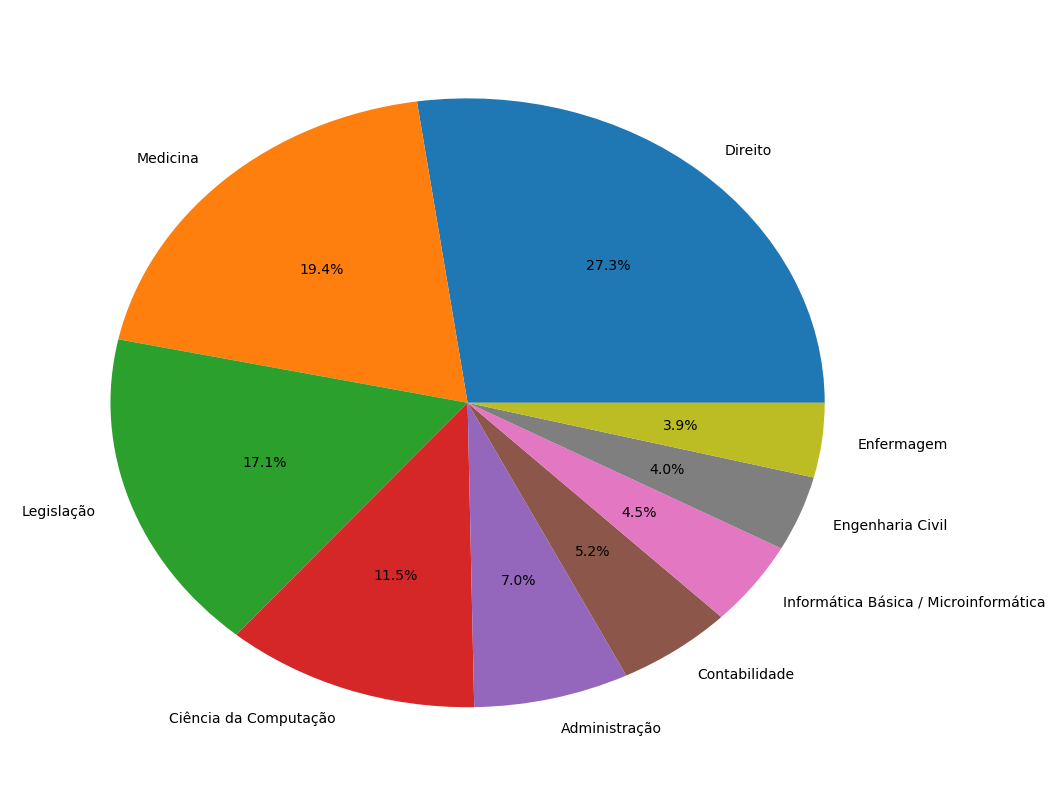
\includegraphics[width=1.0\textwidth]{figures/pie_graph.png}
	\caption{Distribuição das categorias selecionadas}
	\label{fig:pie_labels_graph}
\end{figure}

\section{Seleção dos Modelos}

Uma grande influência na escolha dos modelos em que foi dado um maior foco de otimização foi o guia de classificação de texto produzido por \cite{Text_classification_guide} e ilustrado pelo fluxograma da figura \ref{fig:TextClassificationFlowchart}. Esse guia se trata do resultado de anos de pesquisa em que foram executados cerca de 450 mil experimentos para avaliar a performance de diversos modelos com diferentes hiperparâmetros e conjuntos de dados. Assim, ele tem como objetivo evitar esforços redundantes na seleção e no treinamento de modelos em novos conjuntos de dados.

\begin{figure}[!ht]
	\centering
	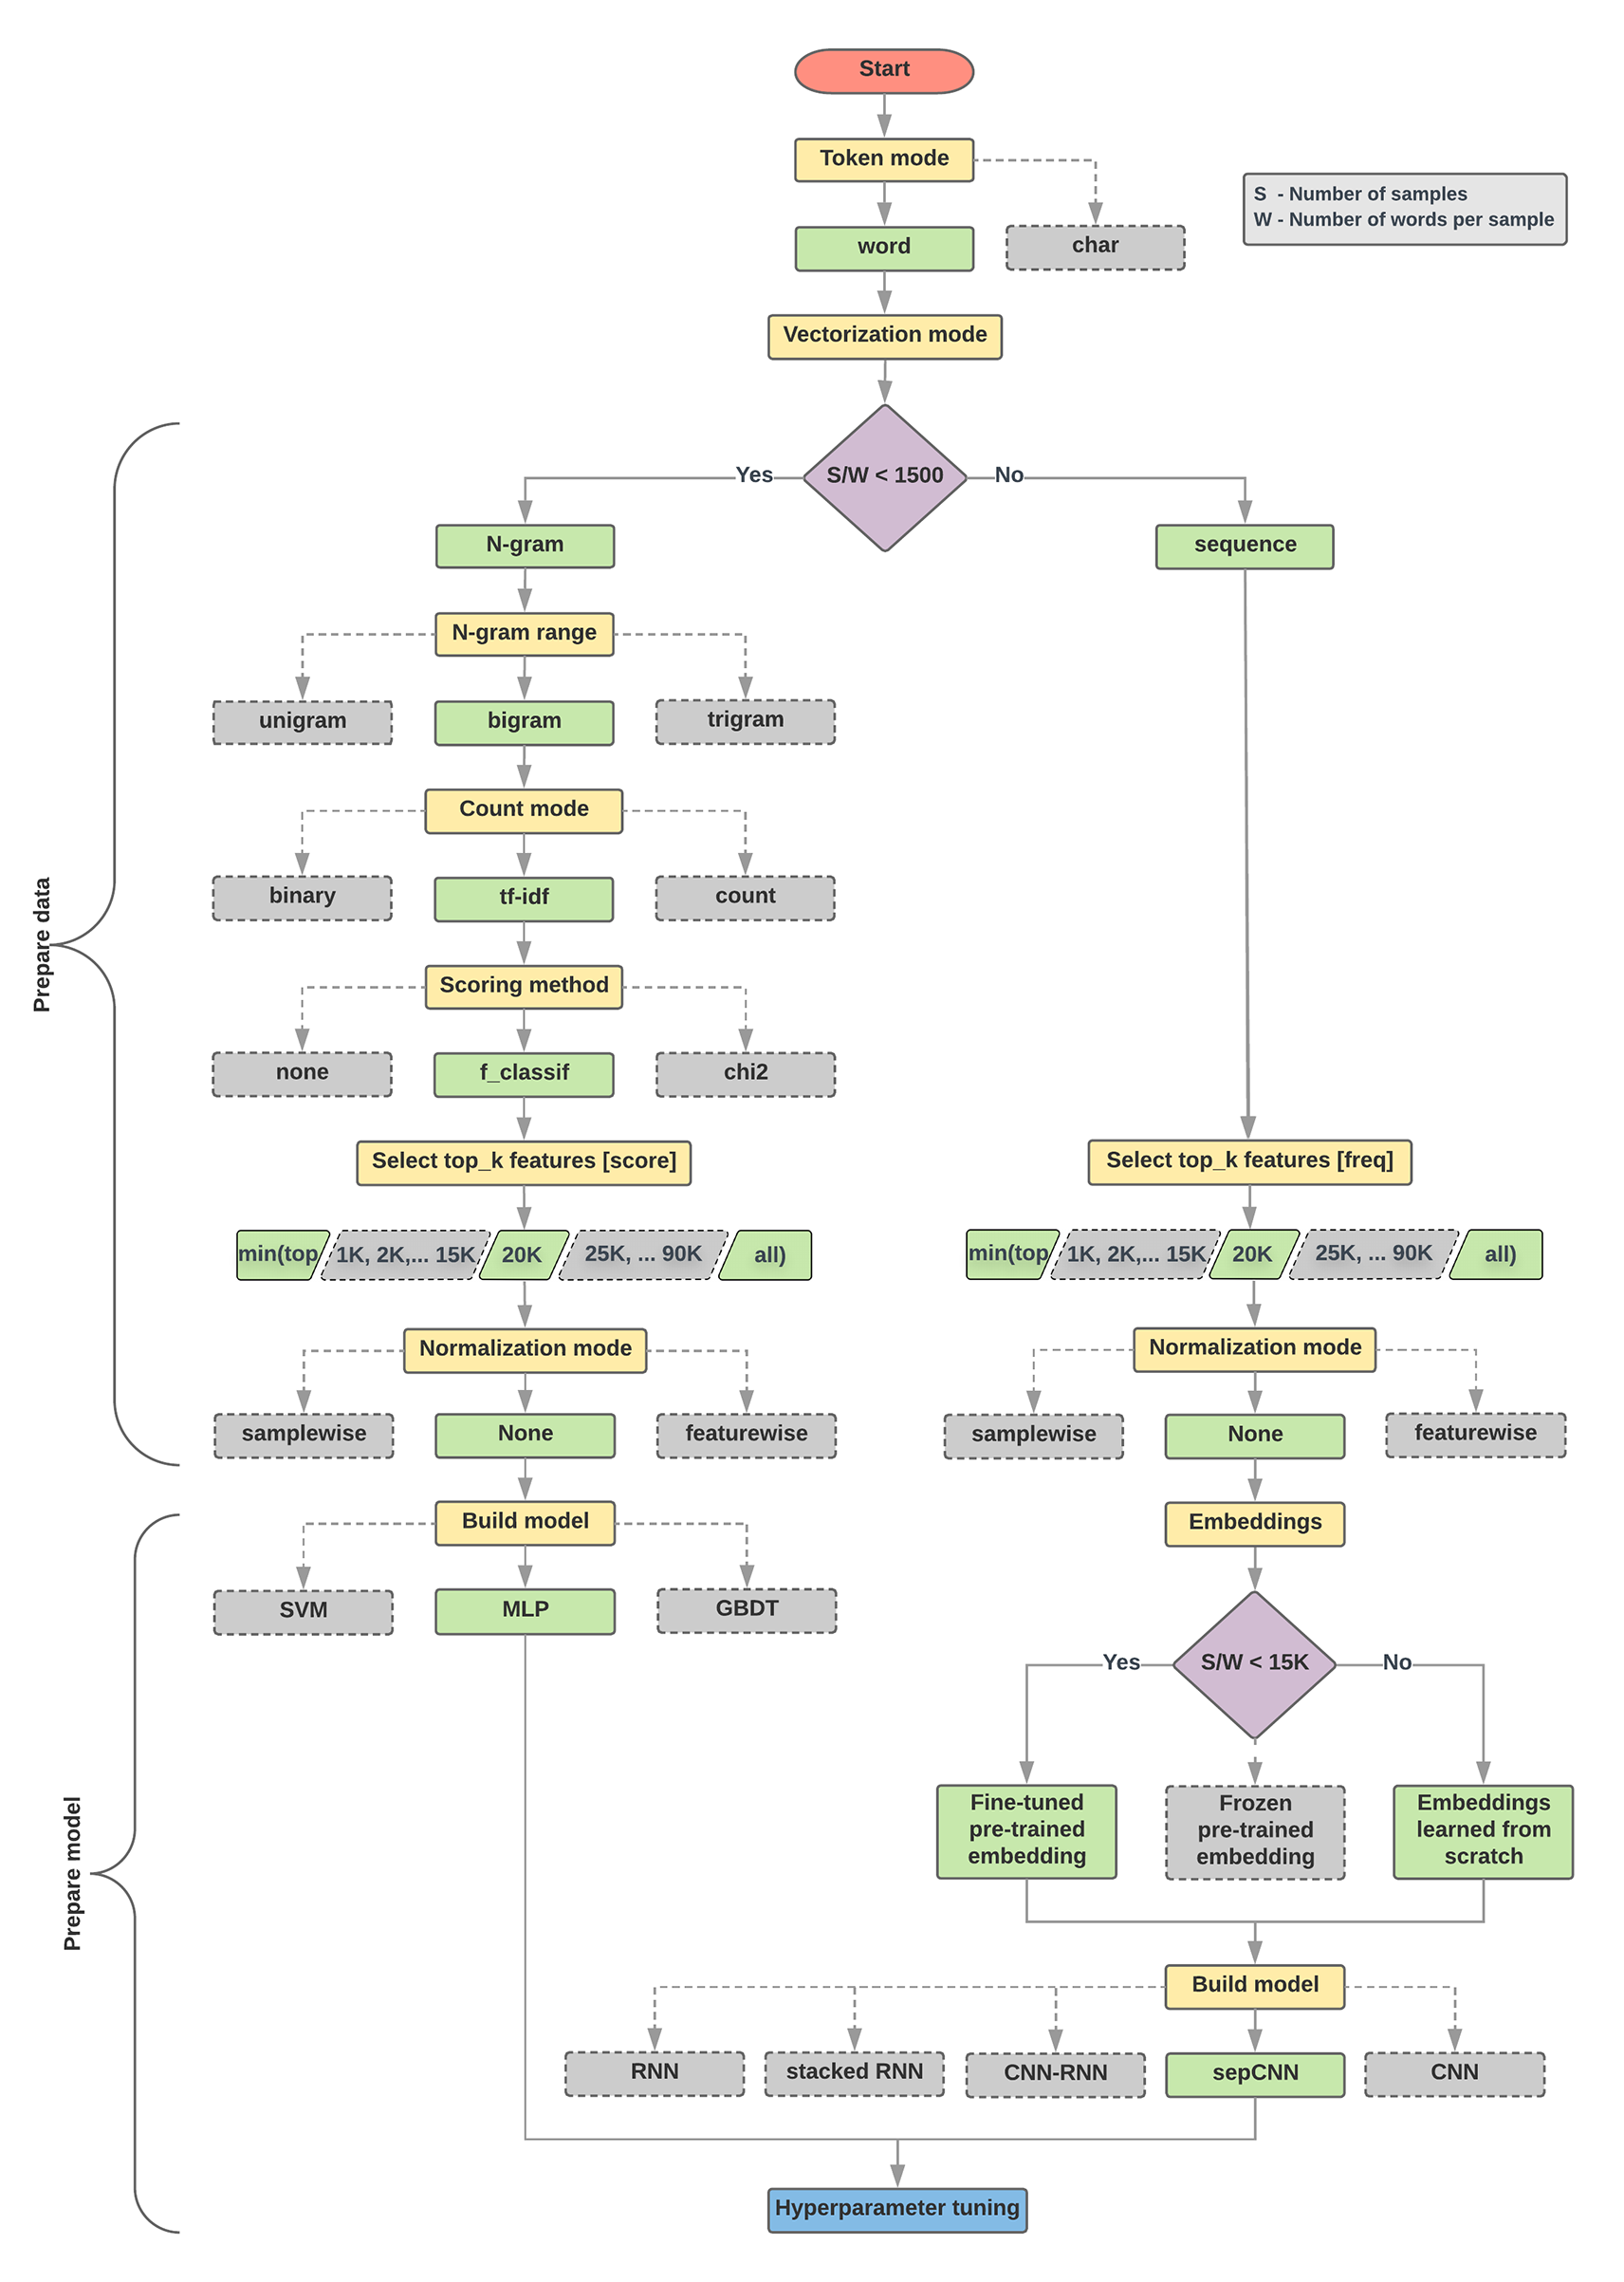
\includegraphics[width=1.0\textwidth]{figures/TextClassificationFlowchart.png}
	\caption{Fluxograma para classificação de texto (fonte: \cite{Text_classification_guide})}
	\label{fig:TextClassificationFlowchart}
\end{figure}

O fluxograma da figura \ref{fig:TextClassificationFlowchart} é baseado na correlação encontrada na razão entre o número de amostras do conjunto de dados (S) e a mediana do comprimento do texto de cada uma dessas questões (W) para a tomada de decisão em suas bifurcações na busca por uma acurácia ótima. No presente trabalho, a partir dos parâmetros da API de dados já definidos, tem-se um total de 299.314 amostras e uma mediana de 65 palavras por amostra, resultando em uma razão (S/W) de aproximadamente 4604.83. Assim, o modelo mais recomendado é o sequencial com o uso de \textit{word embedding} conforme ilustra a figura ref{fig:TextClassificationFlowchart}. Além disso, recomenda-se também o treinamento de uma camada de \textit{embedding} que parta de um modelo pré-treinado, pois um treinamento a partir de valores aleatórios exigiria uma maior razão S/W.

O presente trabalho não se restringe a modelos sequenciais. Implementou-se também modelos baseados em n-gramas, pois estes são modelos mais simples e tradicionais que atuam como bons pontos de referência na comparação dos resultados finais. Contudo, após uma avaliação inicial dos resultados, as recomendações do guia (por \cite{Text_classification_guide}) se confirmaram e os modelos sequenciais mostraram melhores resultados. Por essa razão, em iterações posteriores dos modelos, apenas os sequenciais foram explorados na busca por hiperparâmetros que correspondessem a melhores resultados.